\documentclass[11pt,a4paper]{article}
\usepackage[margin=2.2cm]{geometry}
\usepackage{graphicx}
\usepackage{booktabs}
\usepackage{siunitx}
\usepackage{pgfplots}
\pgfplotsset{compat=1.18}
\usepackage{listings}
\usepackage{xcolor}
\usepackage{caption}
\usepackage{subcaption}
\usepackage{hyperref}
\usepackage{float}
\usepackage{enumitem}
\usepackage{multicol}
\usepackage{tikz}
\usetikzlibrary{shapes.geometric, arrows.meta, positioning, fit}

\lstset{
    language=C,
    basicstyle=\ttfamily\scriptsize,
    keywordstyle=\color{blue},
    commentstyle=\color{gray},
    numbers=left,
    numberstyle=\tiny,
    breaklines=true,
    frame=single,
    tabsize=4,
    extendedchars=true,
    inputencoding=utf8,
    literate={—}{{---}}3 {→}{{$\rightarrow$}}1
}

\title{\vspace{-1.5cm}\textbf{FPGA Kernel Optimization}\\
\large Advanced Computer Architecture -- Lab 3.4\\[0.3em]
\normalsize Summer Semester 2026 \,|\, \"Ubung 1 \,|\, Group 1}
\author{Daniel Wilger (4757813) \and Daniel Bayer (4760237) \and Arjan Siddhpura (3707267)}
\date{\vspace{-0.5cm}}

\begin{document}
\maketitle
\vspace{-0.5cm}

\section{Hardware Platform}

The system is built on the Zybo Z7 FPGA board featuring a Xilinx Zynq-7000 SoC. The MicroBlaze soft processor is instantiated in programmable logic with a configurable microarchitecture. Figure~\ref{fig:blockdiagram} shows the block diagram.

\begin{figure}[H]
    \centering
    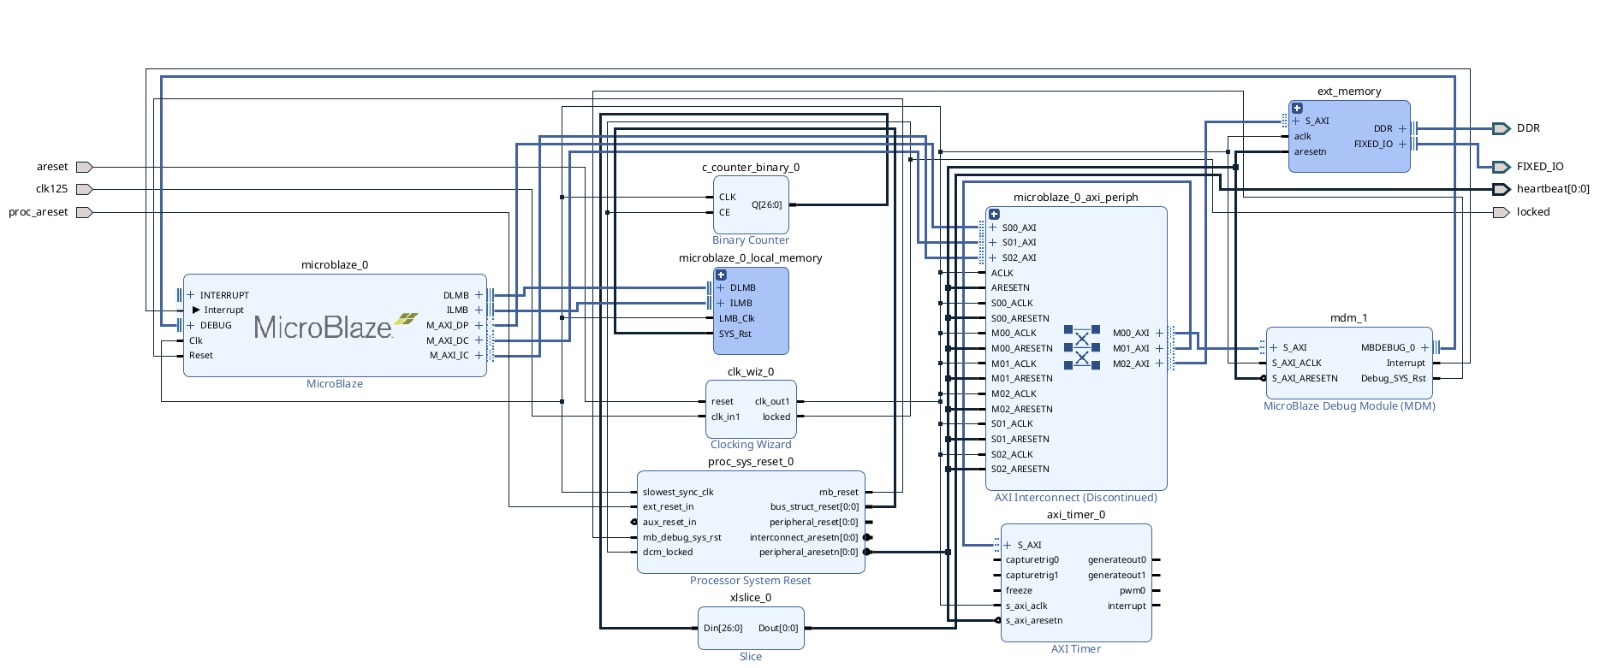
\includegraphics[width=\textwidth]{PHOTO-2026-06-22-12-43-21.jpg}
    \caption{Vivado block diagram: MicroBlaze with local memory, AXI interconnect, DDR3 external memory controller (via ZYNQ PS), AXI Timer, binary counter (heartbeat), and MDM debug module.}
    \label{fig:blockdiagram}
\end{figure}

Two hardware configurations were used to isolate the impact of microarchitectural features:

\begin{table}[H]
\centering
\caption{MicroBlaze configuration comparison}
\label{tab:hwconfig}
\small
\begin{tabular}{lcc}
\toprule
\textbf{Feature} & \textbf{Unoptimized} & \textbf{Optimized} \\
\midrule
Implementation Optimization & Extended (5-stage pipeline) & Extended (5-stage pipeline) \\
Instruction Cache (8\,KB) & Disabled (SW) & Enabled \\
Data Cache (8\,KB) & Disabled (SW) & Enabled \\
Floating Point Unit & None & Extended \\
Integer Multiplier & None & 32-bit (MUL32) \\
Barrel Shifter & Disabled & Enabled \\
Integer Divider & Disabled & Enabled \\
Pattern Comparator & Disabled & Enabled \\
Branch Target Cache & Disabled & 512 entries \\
\bottomrule
\end{tabular}
\end{table}

Both configurations use the 5-stage pipeline (Extended implementation), as this was the default from the initial lab setup. The external DDR3 memory (512\,MB, accessed via the ZYNQ PS HP0 AXI port) stores all program data and code. The heap was configured to 128\,KB in the linker script to accommodate the test arrays.

\section{Methodology}

\subsection{Experimental Design}

To isolate the contribution of each optimization category, five configurations were tested per kernel, progressively enabling optimizations:

\begin{enumerate}[noitemsep]
    \item \textbf{Baseline}: \texttt{-O0}, original code, hardware unoptimized
    \item \textbf{Compiler}: \texttt{-O2}, original code, hardware unoptimized
    \item \textbf{Hardware}: \texttt{-O0}, original code, hardware optimized
    \item \textbf{Software}: \texttt{-O0}, optimized code, hardware optimized
    \item \textbf{All combined}: \texttt{-O3}, optimized code, hardware optimized
\end{enumerate}

This progression reveals: compiler-only gains (1$\to$2), hardware-only gains (1$\to$3), software restructuring gains (3$\to$4), and the synergistic combination (1$\to$5). An additional test without the FPU was performed for Kernel~4 to quantify the FPU impact on floating-point workloads.

\subsection{Measurement Protocol}

Execution time was measured using the AXI Timer (64-bit counter at the MicroBlaze core clock frequency). Before each measurement, \texttt{Xil\_DCacheInvalidate()} ensures a cold-cache start for fair comparison. Array size is 4096 elements for all kernels (128 for Kernel~2 to prevent overflow). All arrays are allocated on DDR3 via \texttt{malloc()} and initialized with pseudo-random data (\texttt{srand(42)}). Most measurements were performed as single runs; spot-checked repetitions showed variation below 0.0001\,s, confirming high reproducibility of the AXI Timer on this deterministic (no-OS) platform.

\subsection{Software Optimization Strategy}

Figure~\ref{fig:flowchart} summarizes the optimization approach applied to each kernel.

\begin{figure}[H]
\centering
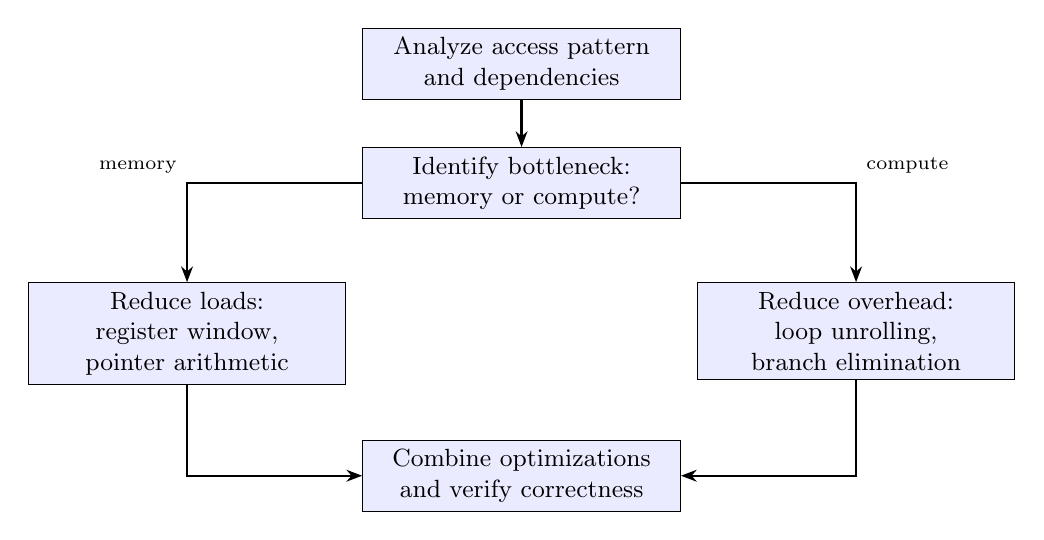
\begin{tikzpicture}[
    node distance=0.6cm and 0.3cm,
    block/.style={rectangle, draw, fill=blue!8, text width=3.8cm, minimum height=0.7cm, align=center, font=\small},
    arrow/.style={-{Stealth[length=2mm]}, thick}
]
\node[block] (analyze) {Analyze access pattern\\and dependencies};
\node[block, below=of analyze] (identify) {Identify bottleneck:\\memory or compute?};
\node[block, below left=0.8cm and 0.2cm of identify] (memopt) {Reduce loads:\\register window,\\pointer arithmetic};
\node[block, below right=0.8cm and 0.2cm of identify] (compopt) {Reduce overhead:\\loop unrolling,\\branch elimination};
\node[block, below=2.8cm of identify] (combine) {Combine optimizations\\and verify correctness};

\draw[arrow] (analyze) -- (identify);
\draw[arrow] (identify) -| node[above left, font=\scriptsize]{memory} (memopt);
\draw[arrow] (identify) -| node[above right, font=\scriptsize]{compute} (compopt);
\draw[arrow] (memopt) |- (combine);
\draw[arrow] (compopt) |- (combine);
\end{tikzpicture}
\caption{Kernel optimization decision flow.}
\label{fig:flowchart}
\end{figure}

\textbf{Kernel 1} (\texttt{A[i] += A[i+offset]}): Stride-1 access pattern, memory-bound. Optimized with pointer arithmetic (eliminates index scaling) and 4$\times$ loop unrolling (reduces branch overhead by 75\%).

\textbf{Kernel 2} (\texttt{A[i] = A[i-1] + A[i-2]*A[i-3]}): Serial loop-carried dependency limits parallelism. Optimized with a register sliding window that eliminates 2 of 3 loads per iteration by keeping \texttt{A[i-1]}, \texttt{A[i-2]}, \texttt{A[i-3]} in registers, plus 2$\times$ unrolling.

\textbf{Kernel 3} (\texttt{h[idx[i]] += w[i]}): Indirect (scatter) access causes random cache misses on \texttt{h[]}. Two variants: (A) 4$\times$ unrolling with register-cached indices, and (B) sorting \texttt{idx[]} for sequential access to \texttt{h[]}.

\textbf{Kernel 4} (\texttt{sum += diff if diff > 0}): Data-dependent branch ($\sim$50\% taken with random data). Optimized with branchless accumulation (\texttt{sum += (d > 0) ? d : 0}), 4 independent accumulators to hide FPU latency, and 4$\times$ loop unrolling.

\section{Results}

Table~\ref{tab:results} presents all measured execution times and speedups relative to the baseline. The ``No FPU'' row isolates the FPU contribution by disabling only the FPU while keeping all other hardware optimizations enabled.

\begin{table}[H]
\centering
\caption{Execution times (seconds) and speedup ($\times$ vs.\ baseline) for each kernel.}
\label{tab:results}
\small
\setlength{\tabcolsep}{3.5pt}
\begin{tabular}{l cc cc cc cc}
\toprule
 & \multicolumn{2}{c}{\textbf{Kernel 1}} & \multicolumn{2}{c}{\textbf{Kernel 2}} & \multicolumn{2}{c}{\textbf{Kernel 3}} & \multicolumn{2}{c}{\textbf{Kernel 4}} \\
\cmidrule(lr){2-3}\cmidrule(lr){4-5}\cmidrule(lr){6-7}\cmidrule(lr){8-9}
\textbf{Configuration} & Time & S$\uparrow$ & Time & S$\uparrow$ & Time & S$\uparrow$ & Time & S$\uparrow$ \\
\midrule
1. Baseline          & 0.0567 & 1.0  & 0.00916 & 1.0  & 0.5706 & 1.0  & 44.07  & 1.0 \\
2. Compiler          & 0.0159 & 3.6  & 0.00738 & 1.2  & 0.5177 & 1.1  & 1.092  & 40 \\
3. Hardware          & 0.00230 & 25  & 0.000092 & 100 & 0.00369 & 155 & 0.00304 & 14{,}479 \\
4. Software          & 0.00268 & 21  & 0.000122 & 75  & 0.00341 & 167 & 0.00313 & 14{,}081 \\
5. All combined      & 0.00138 & 41  & 0.000025 & 366 & 0.00186 & 307 & 0.00176 & 25{,}084 \\
\midrule
6. No FPU (HW opt)   & \multicolumn{2}{c}{N/A} & \multicolumn{2}{c}{N/A} & 0.01621 & 35 & 0.03091 & 1{,}426 \\
\bottomrule
\end{tabular}
\end{table}

\vspace{-0.2cm}
\noindent The FPU alone accounts for a 10.2$\times$ speedup on Kernel~4 (comparing rows 3 and 6), confirming that software floating-point emulation is the single largest bottleneck for FP-heavy workloads.

\begin{figure}[H]
\centering
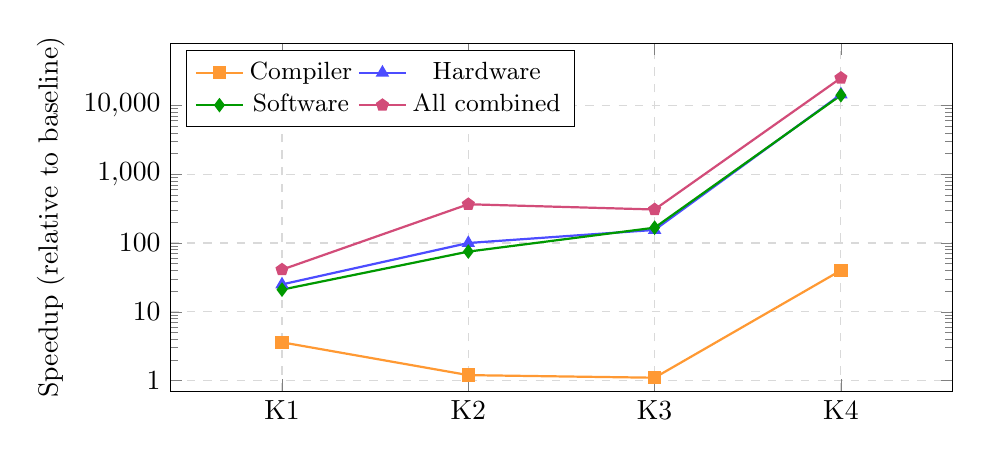
\begin{tikzpicture}
\begin{axis}[
    width=0.95\textwidth,
    height=6cm,
    ymode=log,
    ylabel={Speedup (relative to baseline)},
    symbolic x coords={K1, K2, K3, K4},
    xtick=data,
    legend style={at={(0.02,0.98)}, anchor=north west, legend columns=2, font=\small},
    ymin=0.7,
    ymax=80000,
    enlarge x limits=0.2,
    log ticks with fixed point,
    ytick={1,10,100,1000,10000},
    grid=major,
    grid style={dashed, gray!30},
]
\addplot[mark=square*, thick, orange!80] coordinates {(K1,3.6) (K2,1.2) (K3,1.1) (K4,40)};
\addplot[mark=triangle*, thick, blue!70] coordinates {(K1,25) (K2,100) (K3,155) (K4,14479)};
\addplot[mark=diamond*, thick, green!60!black] coordinates {(K1,21) (K2,75) (K3,167) (K4,14081)};
\addplot[mark=pentagon*, thick, purple!70] coordinates {(K1,41) (K2,366) (K3,307) (K4,25084)};
\legend{Compiler, Hardware, Software, All combined}
\end{axis}
\end{tikzpicture}
\caption{Speedup relative to baseline (log scale). Hardware optimization dominates; the compiler alone provides limited improvement. The combination of all three approaches yields the highest overall speedup.}
\label{fig:speedup}
\end{figure}

\section{Discussion}

\subsection{Hardware Dominates Performance}

The most striking result is that hardware optimization alone (config 1$\to$3) yields speedups of 25--14{,}479$\times$, dwarfing compiler-only improvements (1--40$\times$). This demonstrates that the memory hierarchy is the primary performance bottleneck: without caches, every load/store incurs $\sim$30+ cycle DDR3 latency, making even simple loops extremely slow. Kernel~4 shows the most extreme case (14{,}479$\times$) because it combines two effects: the FPU eliminates software floating-point emulation ($\sim$10$\times$) and the cache eliminates $\sim$4096 DDR3 accesses per array ($\sim$1400$\times$).

To isolate the compute-unit contribution from caches, we also measured with full HW optimization but caches disabled. Kernel~2 achieved 29$\times$ speedup (0.007166\,s $\to$ 0.000248\,s) purely from the hardware multiplier, and Kernel~4 achieved 71$\times$ (1.092\,s $\to$ 0.0154\,s) from the FPU alone. This confirms that compute units and caches address fundamentally different bottlenecks: arithmetic throughput vs.\ memory latency.

\subsection{Compiler Optimization Without Cache Is Limited}

Configuration~2 shows that \texttt{-O2} provides only moderate improvement without caches (K2: 1.2$\times$, K3: 1.1$\times$). The compiler can schedule instructions optimally, but when every load stalls for 30+ cycles, instruction-level improvements are overwhelmed by memory latency. The notable exception is K4 (40$\times$), where the compiler replaces software FP emulation library calls with inlined sequences. This confirms that \textbf{compiler optimization cannot overcome the memory wall without hardware support}.

\subsection{Software Optimization: Context-Dependent}

An unexpected finding: at \texttt{-O0} with full hardware optimization, the software-optimized code is marginally \emph{slower} for K1 and K2 (configs 3 vs.\ 4). This occurs because at \texttt{-O0}, the additional local variables (pointer temporaries, register window values) are placed on the stack rather than in registers, adding overhead. However, when combined with \texttt{-O3} (config 5), the compiler can fully utilize the restructured code, yielding the best overall performance.

A further subtlety: at \texttt{-O3} with full HW, Kernel~1's optimized code is actually \emph{slower} than the baseline (0.00138\,s vs.\ 0.00114\,s, speedup 0.83$\times$). This demonstrates that \texttt{-O3} already applies the same loop unrolling and pointer optimizations automatically. The hand-optimized code then adds redundant structure that the compiler cannot fully simplify, resulting in a net negative. This reinforces that manual software optimization is most valuable at low optimization levels or when caches are absent.

Crucially, when caches are \emph{disabled} but other HW features are present, the software optimizations provide significant gains (K1: 1.79$\times$, K2: 1.70$\times$ at \texttt{-O0}), because each eliminated load saves 30+ cycles of DDR3 latency. This confirms the optimizations are correctly targeted at memory access reduction.

\subsection{Why Some Kernels Are Easier to Optimize}

\noindent\textbf{Kernel 1} (easiest): Regular stride-1 access pattern benefits enormously from caching and unrolling. No dependencies between iterations allow full exploitation of all optimization techniques.

\noindent\textbf{Kernel 2} (hardest for software): The loop-carried dependency (\texttt{A[i]} depends on \texttt{A[i-1]}) fundamentally limits parallelism. However, the register sliding window is highly effective because it targets loads, not computation.

\noindent\textbf{Kernel 3}: The indirect access pattern makes this kernel cache-hostile. The sort-based optimization (variant B) was counterproductive: O($n^2$) insertion sort on 4096 elements costs far more than it saves, since \texttt{h[]} (4\,KB) fits entirely in the 8\,KB data cache. The unrolled variant provides modest improvement by reducing branch overhead on the sequential \texttt{idx[]}/\texttt{w[]} accesses.

\noindent\textbf{Kernel 4}: Benefits most dramatically from hardware (FPU + cache). The branchless optimization shines at \texttt{-O3} with BTC enabled (1.46$\times$), showing that software branch elimination and hardware branch prediction address the same bottleneck from different angles.

\subsection{Key Takeaway}

The optimal strategy is a combination of all three layers: hardware provides the foundation (cache, FPU, BTC), software restructuring reduces unnecessary work (register reuse, branch elimination), and the compiler translates well-structured code into efficient machine instructions. No single layer is sufficient alone.

\newpage
\appendix
\section{Additional Figures}

Figure~\ref{fig:perkernel_log} shows execution times for all four kernels on a shared logarithmic y-axis. A shared axis enables direct cross-kernel comparison: after full optimization, all kernels converge to similar magnitudes ($\sim$1\,ms), despite baselines spanning three orders of magnitude.

\begin{figure}[H]
\centering
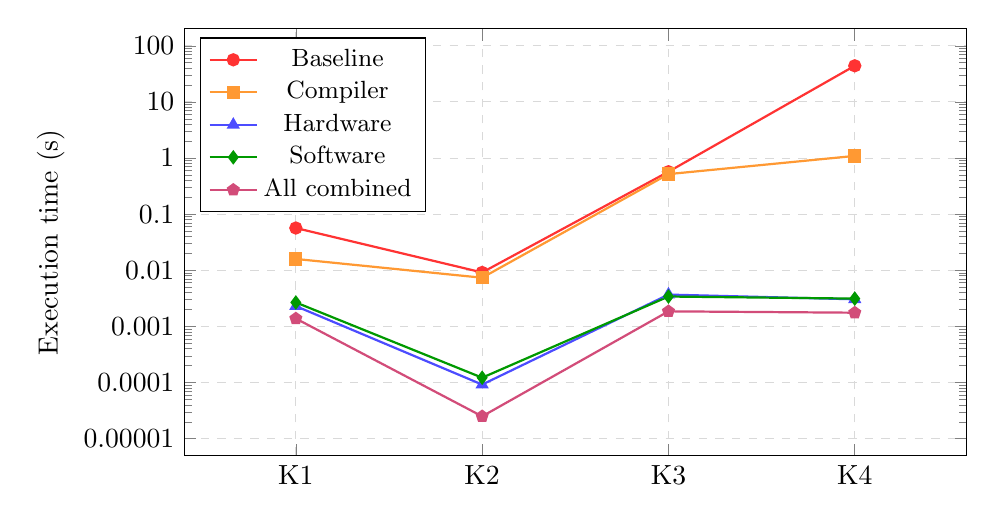
\begin{tikzpicture}
\begin{axis}[
    width=0.95\textwidth,
    height=7cm,
    ymode=log,
    ylabel={Execution time (s)},
    symbolic x coords={K1, K2, K3, K4},
    xtick=data,
    legend style={at={(0.02,0.98)}, anchor=north west, legend columns=1, font=\small},
    ymin=0.000005,
    ymax=200,
    enlarge x limits=0.2,
    log ticks with fixed point,
    ytick={0.00001, 0.0001, 0.001, 0.01, 0.1, 1, 10, 100},
    grid=major,
    grid style={dashed, gray!30},
]
\addplot[mark=*, thick, red!80] coordinates {(K1,0.056679) (K2,0.009158) (K3,0.570567) (K4,44.071876)};
\addplot[mark=square*, thick, orange!80] coordinates {(K1,0.015929) (K2,0.007375) (K3,0.517663) (K4,1.092015)};
\addplot[mark=triangle*, thick, blue!70] coordinates {(K1,0.002302) (K2,0.000092) (K3,0.003692) (K4,0.003044)};
\addplot[mark=diamond*, thick, green!60!black] coordinates {(K1,0.002677) (K2,0.000122) (K3,0.003412) (K4,0.003133)};
\addplot[mark=pentagon*, thick, purple!70] coordinates {(K1,0.001382) (K2,0.000025) (K3,0.001857) (K4,0.001757)};
\legend{Baseline, Compiler, Hardware, Software, All combined}
\end{axis}
\end{tikzpicture}
\caption{Execution times across all kernels (shared log scale). Higher points indicate slower execution. All kernels converge to $\sim$1--2\,ms after full optimization, despite baselines spanning three orders of magnitude.}
\label{fig:perkernel_log}
\end{figure}

\begin{figure}[H]
\centering
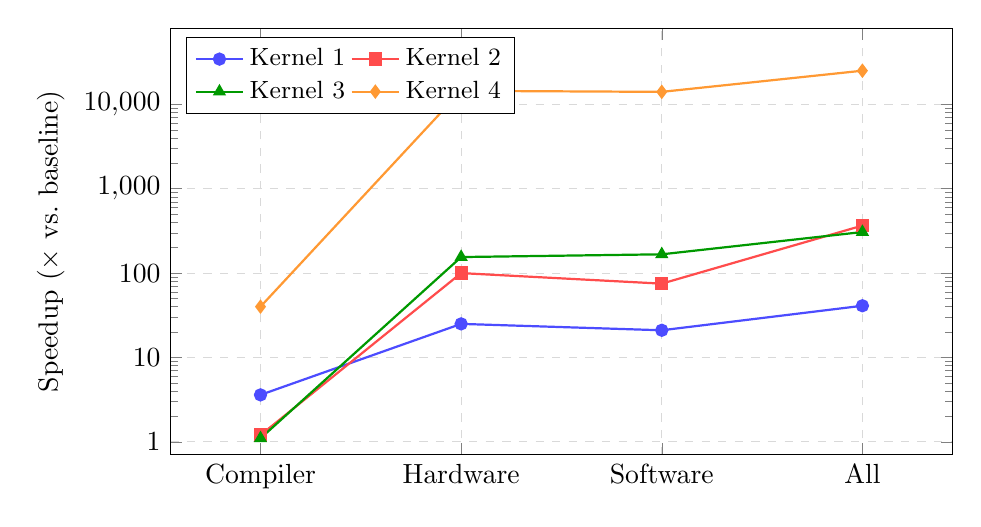
\begin{tikzpicture}
\begin{axis}[
    width=0.95\textwidth,
    height=7cm,
    ymode=log,
    ylabel={Speedup ($\times$ vs.\ baseline)},
    symbolic x coords={Compiler, Hardware, Software, All},
    xtick=data,
    legend style={at={(0.02,0.98)}, anchor=north west, legend columns=2, font=\small},
    ymin=0.7,
    ymax=80000,
    enlarge x limits=0.15,
    log ticks with fixed point,
    ytick={1, 10, 100, 1000, 10000},
    grid=major,
    grid style={dashed, gray!30},
]
\addplot[mark=*, thick, blue!70] coordinates {(Compiler,3.6) (Hardware,25) (Software,21) (All,41)};
\addplot[mark=square*, thick, red!70] coordinates {(Compiler,1.2) (Hardware,100) (Software,75) (All,366)};
\addplot[mark=triangle*, thick, green!60!black] coordinates {(Compiler,1.1) (Hardware,155) (Software,167) (All,307)};
\addplot[mark=diamond*, thick, orange!80] coordinates {(Compiler,40) (Hardware,14479) (Software,14081) (All,25084)};
\legend{Kernel 1, Kernel 2, Kernel 3, Kernel 4}
\end{axis}
\end{tikzpicture}
\caption{Per-kernel speedup by optimization type (shared log scale). Kernel~4 gains the most from hardware (FPU), while Kernel~2 shows the strongest all-combined multiplier due to HW multiplier, caches, and register optimization together.}
\label{fig:speedup_perkernel}
\end{figure}

%% =============================================================
%% Source Code Appendix (commented out for now)
%% =============================================================
% \section{Source Code}
%
% \subsection{Main Test Harness}
% \lstinputlisting{src/main.c}
%
% \subsection{Kernel 1 -- Optimized}
% \lstinputlisting{src/kernel1_optimized.c}
%
% \subsection{Kernel 2 -- Optimized}
% \lstinputlisting{src/kernel2__optimized.c}
%
% \subsection{Kernel 3 -- Optimized}
% \lstinputlisting[firstline=1,lastline=162]{src/kernel3._optimized.c}
%
% \subsection{Kernel 4 -- Optimized}
% \lstinputlisting{src/kernel4_optimized.c}

\end{document}
